\documentclass[10pt, conference]{IEEEtran}
\IEEEoverridecommandlockouts
% The preceding line is only needed to identify funding in the first footnote. If that is unneeded, please comment it out.
\usepackage{cite}
\usepackage{amsmath,amssymb,amsfonts}
\usepackage{algorithmic}
\usepackage{graphicx}
\usepackage{textcomp}
\usepackage{xcolor}
\usepackage{booktabs}
\usepackage{graphicx}
\def\BibTeX{{\rm B\kern-.05em{\sc i\kern-.025em b}\kern-.08em
    T\kern-.1667em\lower.7ex\hbox{E}\kern-.125emX}}
\begin{document}

\title{NodeSRT: a Selective Regression Testing Tool for Node.js Application}

\author{\IEEEauthorblockN{Yufeng Chen}
\IEEEauthorblockA{
\textit{University of British Columbia}\\
Vancouver, Canada \\
yufengcy@student.ubc.ca}
}

\maketitle

\begin{abstract}
Node.js is one of the most popular frameworks for building web applications. As software system 
matures, the cost of running the entire regression test suite becomes significant. 
Selective Regression Testing (SRT) is a technique that by rerunning only a subset of tests, regression test suite can detect software failures more efficiently. 
However, previous SRT studies mainly focused on standard desktop applications. Node.js applications are 
considered hard to perform test reduction because Node's asynchronous, event-driven programming model and 
JavaScript is a dynamic programming language. 
In this paper, we present NodeSRT, a Selective Regression Testing framework for Node.js applications. 
By performing static and dynamic analysis, NodeSRT gets relationship between changed method and their 
relationships with each test, and reduces the whole regression test suite to only tests that are 
affected by change, which would improve the execution time of the regression test suite. 
To evaluate our selection technique, we applied NodeSRT to two open-source projects: Uppy and Simorgh, 
then compared our approach with retest-all strategy and current industry-standard SRT technique: Jest 
OnlyChange option. The results demonstrate that NodeSRT correctly selects affected tests based on 
changes and is 450\% more precise than the Jest OnlyChange option. NodeSRT is also over 2.5 times faster in 
high code coverage project.
    
\end{abstract}

\begin{IEEEkeywords}
JavaScript, Selective Regression Testing, Node.js Application, Static Analysis, Dynamic Analysis
\end{IEEEkeywords}

\section{Introduction}
With the continuous growth of web applications, Node.js has become one of the most popular frameworks 
for web application development \cite{b16}. For critical online services, performing regression testing is important. However, 
since JavaScript is a loosely typed, dynamic language, test 
selection on JavaScript projects is hard. Besides, modern web applications are usually composed of 
more than one component; running unit tests only does not judge the overall behaviour of the web 
application \cite{b8}. 

There are two phases involved in test selection. The first phase is to select tests based on change and 
test dependency graph generated by static or dynamic analysis. The second phase is to run selected tests.
There are four levels of granularity for test selection techniques: statement, method, file, module. The common 
two are method-level and file-level. File-level granularity analysis builds relationship between tests and files in 
the program and selects tests that reflect changed files. Method-level analysis builds relationship between tests and methods 
then selects tests that reflect changed method. Since method-level selection is more complicated than  
file-levle selection, file-level selection runs faster in phase one. However, file-level selection selects more 
tests than needed. Therefore it is less precise than method-level selection and runs slower in phase two. 

Jest OnlyChange is the current industry-standard SRT technique; it operates at file-level granularity and selects 
tests to be rerun based on file changes in the Git repository. As it is safe and the most light-weighted approach. Although fast, this approach may not be precise 
enough for some test suites. Therefore, our research starts from a question:\textit{"Can we find a more 
effective test selection technique for Node.js Applications?"} 

To evaluate effectiveness of test selection technique, Rothermel\cite{b13} proposed four metrics: Inclusiveness, Precision, Efficiency, Generality. Inclusiveness 
measures the extent to which SRT technique chooses tests that are affected by the change. Precision measures 
the ability that SRT technique omits tests that are not affected by the change. Efficiency measures the time and 
space required. Generality measures its ability to function in a comprehensive and practical range of situations.
We say a selection technique is safe if it achieves 100\% inclusiveness.

Our intuition for reducing the total running time is to 
improve the granularity of the selection technique to improve precision so that less tests are required to run in phase two. 
We also evaluated our selection technique by performing an empirical study on two open source Node.js projects in different 
size and code coverage.

\section{Approach Overview}
 Many special language features makes tranditional SRT technique
not working on JavaScript programs. These features include first-class functions, Inheritance and the prototype chain, Asynchronous and Error handling.
To mitigate these challenges, our tool uses a combination of static and dynamic analysis, then perform a modification-based test 
selection algorithm in method level. The Modification-based approach works by analyzing modified code entities 
then select tests based on modifications. This strategy is relatively simple and proved safe by \cite{b3, b4}. NodeSRT can 
also be used in CI/CD environment. NodeSRT consists of five parts: dynamic analysis, static analysis, change analysis, 
test selection, and selected test runner. 
\begin{figure}[htbp]
    \centerline{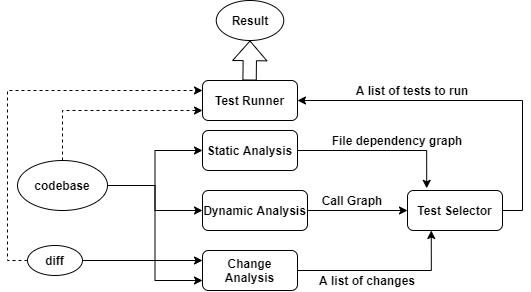
\includegraphics[scale=0.45]{NodeSRT Architecture.png}}
    \caption{NodeSRT Architecture}
    \label{fig}
    \end{figure}    

As shown in Figure 1. The \textbf{Static Analysis module} performs static analysis on original codebase to get file dependency
graph on each tests. It works by identifing and resolving \verb|require| and \verb|import| in JavaScript files. The \textbf{Dynamic Analysis module} generate a dynamic call graph by injecting code to original codebase 
generated AST. Since Node.js applications have the characteristics of client-side, server-side separated, code in 
different modules may be running in a different environment. E.g. The server-side code is running in Node.js 
environment. Client-side code is running in the browser environment. To collect runtime information of both 
modules, NodeSRT uses HTTP requests. The injected code will send logging messages to the server. The logging server will 
collect all the logging messages and generate a call graph in JSON format. As noted by \cite{b2, b4} when the codebase 
becomes large, code analysis result should be store in database to ensure performance. \textbf{Change Analysis module} 
compares the ASTs of the changed files, then generate a JSON representation of changes. Since NodeSRT uses function-level 
granularity, change analysis module finds the closest function name of each different AST node based on their ancestors. 
If the function is anonymous, NodeSRT will generate a unique name for it based on its parent function name, class name and file name. 
This approach is similar to the approach of Chianti \cite{b12} handling anonymous class in Java. With call graph, file dependency graph, 
and JSON representation of changes, \textbf{Test Selector} selects tests affected by changes. To handle changes outside 
functions, the test selector will select tests depend on changed files based on file dependency graph to guarantee safety. 
Finally, The \textbf{Test Runner} will run selected tests.

Our tool can also be used to select end-to-end tests since NodeSRT uses HTTP requests 
record logging messages and build dynamic call graph.

\section{Empirical Evaluation}

To evaluate NodeSRT, we performed empirical evaluation on two open-source Node.js project. We chose these two project because 
our empirical study requires sample has to be well-maintained and has reasonable amount of tests. By using the method mentioned in \cite{b10}, 
we found Uppy and Simorgh. Uppy has 112k lines of code, 216 unit tests and 9 end-to-end tests, 
achieves 20\% of code coverage. Simorgh is the BBC website rebuild using React.js. This project has 698k lines of code. 
It includes 2801 unit tests, achieves 97\% of code coverage. The 
experiment ran on a 4 core x86-64 CPU with 16 GB of RAM, AWS cloud Linux server. Due to the fact that the internet speed and computing speed is not 
unchanged, we use the percentage of tests selected and the percentage of SRT full process running time to 
represent the result. 

\begin{table}[htbp]
    \caption{Empirical study result}
    \centering
    \begin{tabular}{@{}|p{3em}|p{2em}|p{1.8em}|p{3.5em}|p{2em}|p{3.5em}|p{2.5em}|@{}}
    \toprule
    project name & retest time (s)&select time (ms)&NodeSRT test No. (\%)&Jest test No. (\%)& NodeSRT running time (\%) & Jest running time (\%) \\ \midrule
    Uppy         & 69.3  &  490   &                    8.40              &  20.66              &   50.24               &   23.63                    \\ \midrule
    Simorgh      & 450.7  &  2256 &                    2.73              &  17.26              &   8.10                &   30.18                   \\ \bottomrule
    \end{tabular}
    \end{table}



As shown in Table I, given file dependency graph and call graph, the selection step for both project is less than 5\% of total 
running time. Comparing to Jest OnlyChange, NodeSRT selects much less tests for both projects. In fact, NodeSRT selects 1.5 times fewer 
tests in Uppy, 5.32 times fewer tests in Simorgh. Although NodeSRT selects less tests in Uppy, Jest OnlyChange runs faster than NodeSRT. 
This is because Jest OnlyChange makes use of Jest's own jest-haste-map module and customized file system module: watchman. Future works can 
be done for NodeSRT in this part. For project with high code coverage: Simorgh, NodeSRT selectes fewer tests and is 2.72 times faster. 


\section{Related Work and Conclusion}
There are several techniques proposed for standard desktop applications \cite{b2, b3, b4, b5, b7, b9, b12, b13, b14, b17}, most techniques 
first classify prograams into different entities such as functions, types, variables, and macros then utilize comprehensive static analysis 
and dynamic analysis to build entity-tests relationships to reduce test suite.
For studies focused on JavaScript applications, Mutandis \cite{b11} is a generic mutation testing 
approach for JavaScript that guides the mutation generation process. It works by leveraging static and dynamic program 
analysis to guide the mutation generation process a-priori towards parts of the code that are error-prone or 
likely to influence the program’s output. 
Tochal \cite{b1} is a DOM-Sensitive change impact analysis tool for JavaScript. Through dynamic code injection and static analysis, this 
approach incorporates a ranking algorithm for indicating the importance of each entity in the impact set. This 
approach focused on frontend DOM changes, rather than the whole frontend backend interaction. For test selection in different levels 
of granularity, Gligoric \cite{b6} showed that file-level granularity 
analysis runs 32\% faster than the method-level granularity analysis in large scale Java programs.\cite{b15} also shows 
tool implemented with approach "DejaVu" \cite{b14} is 16\% worse when it comes to realistic code-coverage-based test suites.

In this work, we present NodeSRT, a novel approach for performing SRT on Node.js applications in method level. Our empirical evaluation 
showed that our approach outperformed current industry used approach Jest OnlyChange.

\begin{thebibliography}{00}
\bibitem{b1} S. Alimadadi, A. Mesbah and K. Pattabiraman, "Hybrid DOM-Sensitive Change Impact Analysis for JavaScript," in 29th European Conference on Object-Oriented Programming (ECOOP 2015), Dagstuhl, 2015. doi:10.4230/LIPIcs.ECOOP.2015.321.
\bibitem{b2} Á. Beszédes, T. Gergely, L. Schrettner, J. Jász, L. Langó and T. Gyimóthy, "Code coverage-based regression test selection and prioritization in WebKit," in 2012 28th IEEE international conference on software maintenance (ICSM), 2012. pp. 46–55.
\bibitem{b3} S. Biswas, R. Mall, M. Satpathy and S. Sukumaran, "Regression test selection techniques: A survey," Informatica, vol. 35, 2011. 
\bibitem{b4} Y.-F. Chen, D. S. Rosenblum and K.-P. Vo, "TestTube: A system for selective regression testing," in Proceedings of 16th International Conference on Software Engineering, 1994. doi: 10.1109/ICSE.1994.296780.
\bibitem{b5} E. Engström, M. Skoglund and P. Runeson, "Empirical evaluations of regression test selection techniques," in Proceedings of the Second ACM-IEEE international 40 symposium on Empirical software engineering and measurement - ESEM '08, 2008.doi: 10.1145/1414004.1414011.
\bibitem{b6} M. Gligoric, L. Eloussi and D. Marinov, "Practical regression test selection with dynamic file dependencies," in Proceedings of the 2015 International Symposium on Software Testing and Analysis - ISSTA 2015, 2015. doi:10.1145/2771783.2771784.
\bibitem{b7} M. J. Harrold, J. A. Jones, T. Li, D. Liang, A. Orso, M. Pennings, S. Sinha, S. A.Spoon and A. Gujarathi, "Regression test selection for Java software," ACM SIGPLAN Notices, vol. 36, p. 312–326, Nov. 2001. doi: 10.1145/504311.504305.
\bibitem{b8} M. Hirzel, "Selective regression testing for web applications created with google web toolkit," in Proceedings of the 2014 International Conference on Principles and Practices of Programming on the Java platform Virtual machines, Languages, and Tools - PPPJ' 4, 2014. doi: 10.1145/2647508.2647527.
\bibitem{b9} M. J. Harrold and M. L. Souffa, "An incremental approach to unit testing during maintenance," in Proceedings. Conference on Software Maintenance, 1988., 1988. doi: 10.1109/icsm.1988.10188.
\bibitem{b10} A. Labuschagne, L. Inozemtseva and R. Holmes, "Measuring the cost of regression testing in practice: a study of Java projects using continuous integration," Proceedings of the 2017 11th Joint Meeting on Foundations of Software Engineering - ESEC/FSE 2017, 2017, doi: 10.1145/3106237.3106288.
\bibitem{b11} S. Mirshokraie, A. Mesbah and K. Pattabiraman, "Efficient JavaScript Mutation Testing," in 2013 IEEE Sixth International Conference on Software Testing, Verification and Validation, 2013. doi: 10.1109/icst.2013.23.
\bibitem{b12} X. Ren, B. G. Ryder, M. Stoerzer and F. Tip, "Chianti: a change impact analysis tool for Java programs," in Proceedings. 27th International Conference on Software Engineering, 2005. ICSE 2005.. doi: 10.1109/icse.2005.1553643.
\bibitem{b13} G. Rothermel and M. J. Harrold, "Analyzing regression test selection techniques," IEEE Transactions on Software Engineering, vol. 22, p. 529–551, 1996. doi: 10.1109/32.536955.
\bibitem{b14} G. Rothermel and M. J. Harrold, "A safe, efficient regression test selection technique," ACM Transactions on Software Engineering and Methodology (TOSEM), vol. 6, p. 173–210, Apr. 1997. doi: 10.1145/248233.248262.
\bibitem{b15} G. Rothermel and M. J. Harrold, "Empirical studies of a safe regression test selection technique," IEEE Transactions on Software Engineering, vol. 24, p. 401–419, Jun. 1998. doi: 10.1109/32.689399.
\bibitem{b16} F. Schiavio, H. Sun, D. Bonetta, A. Rosà and W. Binder, "NodeMOP: runtime verification for Node.js applications," in Proceedings of the 34th ACM/SIGAPP Symposium on Applied Computing, 2019. doi: 10.1145/3297280.3297456.
\bibitem{b17} A.-B. Taha, S. M. Thebaut and S.-S. Liu, "An approach to software fault localization and revalidation based on incremental data flow analysis," in [1989] Proceedings of the Thirteenth Annual International Computer Software \& Applications Conference. doi: 10.1109/cmpsac.1989.65142.
\end{thebibliography}
\vspace{12pt}

\end{document}
